En este capítulo se realiza una introducción a la Lógica Temporal Lineal, como una extensión de Lógica 
 Proposicional para poder expresar propiedades en sistemas reactivos.
Con esta finalidad, este lenguaje fue introducido por Pnueli en \cite{pnueli}.

La Lógica Lineal Temporal permite expresar propiedades sobre los sistemas en cuestón,
 ya que se agregan operadores que hacen referencia al tiempo y permite representar los distintos estados
 en distintos momentos durante la ejecución del sistema.


\section {Problema}
``{\itshape Se desea implementar un robot autónomo móvil que sea capaz de
hacer la entrega de un pedido en una casa determinada.
  El mismo debe moverse por un escenario e identificar las casas.
  Para recorrer la ruta de entrega, podrá valerse de una línea negra
que representará la calle de la ciudad.

  Las casas estarán ubicadas a un lado de la calle. En el recorrido
se encuentran varias casas, el robot deberá entregar un pedido
en la quinta casa por la que pase.

  El robot deberá pasar por alto las casas anteriores y
al llegar a la casa objetivo debe detenerse totalmente.

  Para probar la solución, se armará un escenario que consiste de
un piso blanco con una línea negra que puede tener curvas.

  Al lado derecho de la línea se ubicarán cajas a menos de 30
centímetros representando las casas.}''




\section {Solución}

  Se armó un robot móvil que cuenta con 3 sensores:

\begin{itemize}
\item Sensor de grises izquierdo
\item Sensor de grises derecho
\item Sensor de distancia apuntando hacia la derecha
\end{itemize}

  Y 2 actuadores:

\begin{itemize}
\item Motor izquierdo
\item Motor derecho 
\end{itemize}


\begin{figure}[hbtp]
\begin{center}
  \caption{Diagrama del robot móvil
    (realizado utilizando fritzing \cite{fritzing})
  }
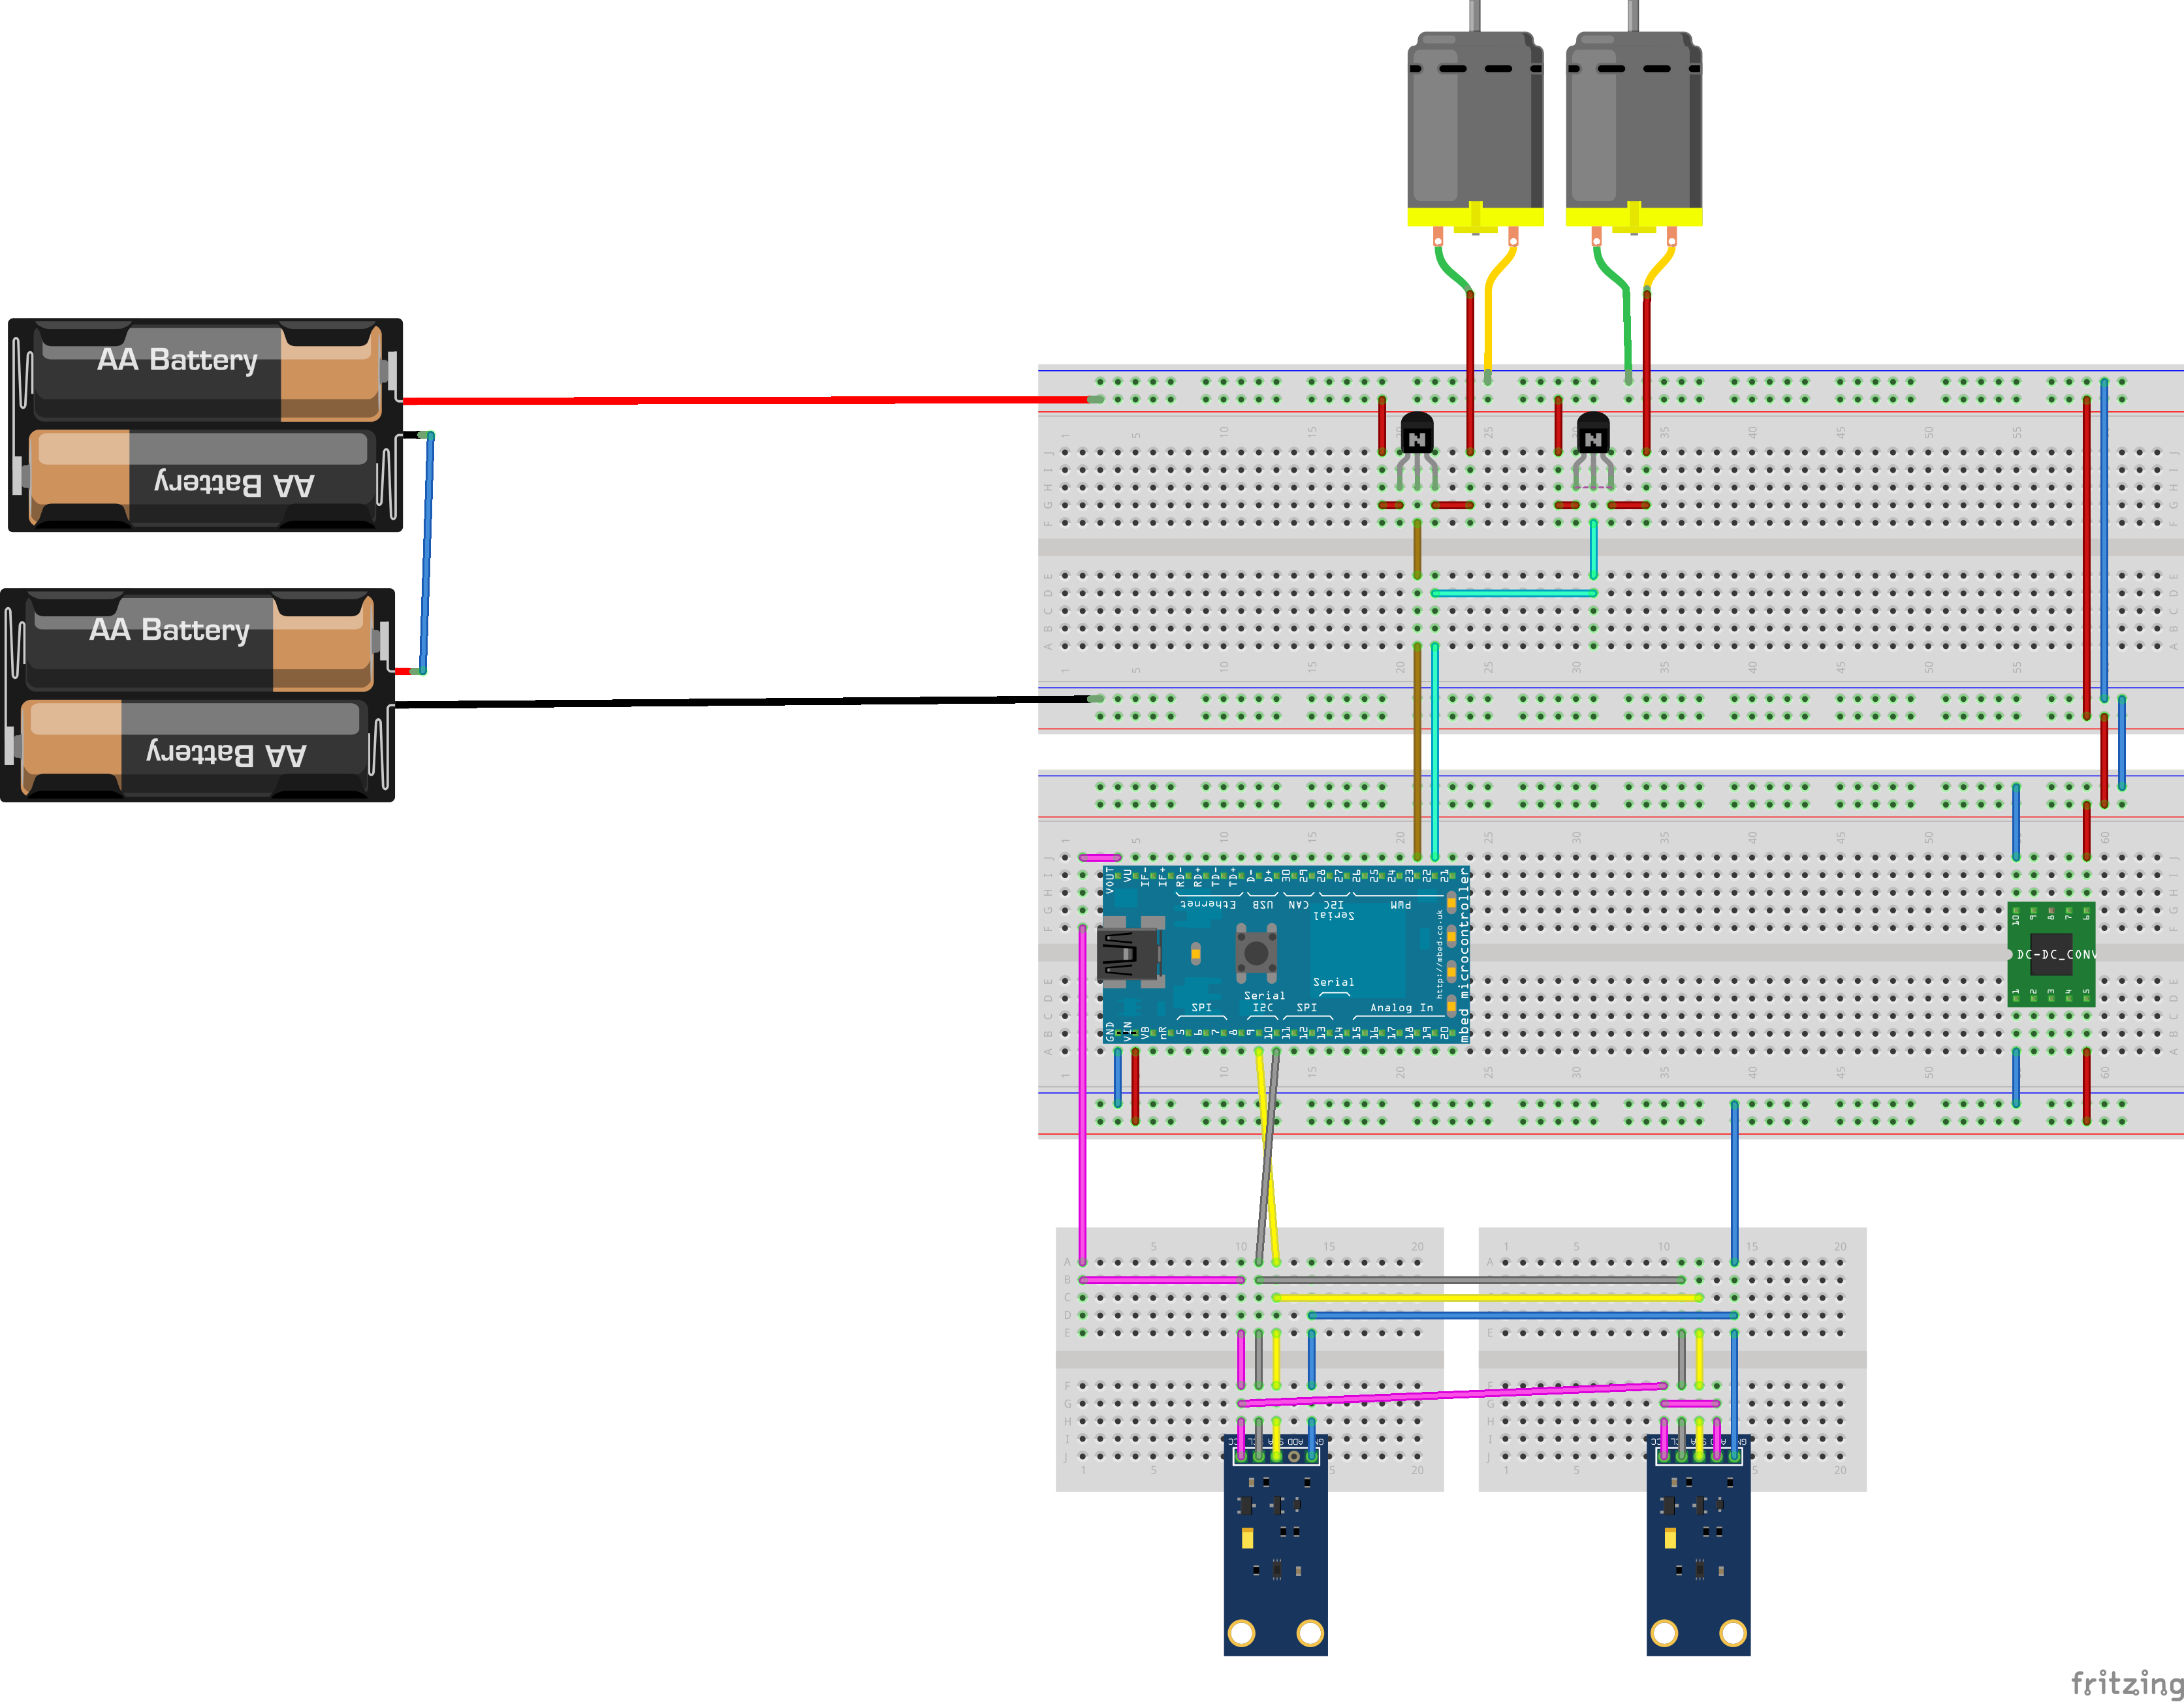
\includegraphics[width=0.9\textwidth]{graphs/breaboardbb.png}
\label{fig:breadboard}
\end{center}
\end{figure}




  El diagrama de la Figura \ref{fig:breadboard} muestra los
componentes físicos que son montados en el robot
para resolver el problema y cómo se interconectan.
  Arriba se pueden ver los dos motores, que irán uno a cada lado
del robot y sólo se moverán hacia adelante.
  Se utilizan salidas \textit{pwm} \footnote{PWM: Del inglés, pulse width
modulation; Modulación por ancho de pulsos. Se utiliza para crear señales
de voltaje en ciclos periódicos y controlar la cantidad de energía que
se envía.} del MBED para controlar la velocidad de cada motor.

  Los motores necesitan más energía que la que se puede entregar con
los pines de salida del MBED, y para ésto tienen su propia fuente de
voltaje.
  Se utilizan dos transistores para amplificar la señal que
controla cada motor.

  El robot utilizará dos sensores de grises montados al frente
para mantenerse sobre la línea, ambos pueden verse a la derecha abajo
en la Figura \ref{fig:breadboard}.
  Con los motores el robot se moverá hacia adelante inicialmente, e
irá corrigiendo su dirección desacelerando el motor del lado que
se salga de la línea.
  Junto a cada sensor de grises se montará una luz led, que de acuerdo
al color del suelo, se reflejará y se podrá decidir si se está viendo
algo oscuro (la línea) o algo claro (fuera de la línea).

  El sensor de distancia a la izquierda debajo en la figura, se montará
en el robot apuntando hacia la derecha, para saber cuándo el mismo
está pasando frente a una casa.

  Durante el trayecto se mantendrá la cuenta de las casas, y el robot
se detendrá totalmente cuando la cuenta llegue al valor 5.

  En la Figura \ref{fig:robotfisico} se puede ver el
robot físico creado como prototipo para probar el caso de estudio.

\begin{figure}[!htb]
\begin{center}
\caption{Robot físico implementado}
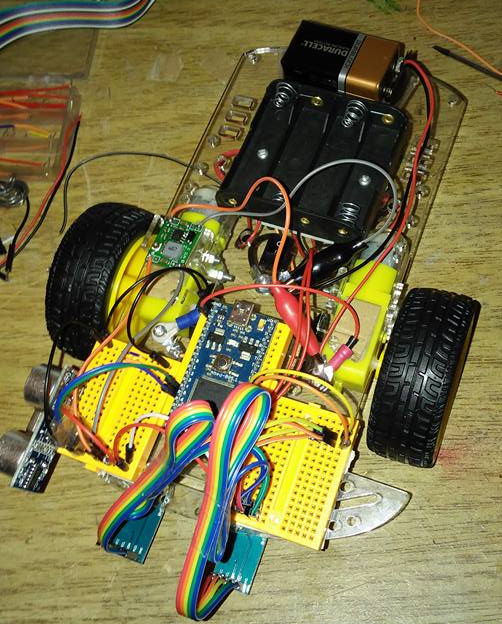
\includegraphics[width=0.9\textwidth]{graphs/alf.jpg}
\label{fig:robotfisico}
\end{center}
\end{figure}




\newpage
\subsection{Implementación usando \frob{}}
  Luego se llega a la implementación en el lenguaje \frob{}:

\begin{verbatim}

INPUT_DISTANCE = 1
INPUT_COLOR_LEFT = 2
INPUT_COLOR_RIGHT = 3
OUTPUT_ENGINE_LEFT = 1
OUTPUT_ENGINE_RIGHT = 2

MIN_DISTANCE = 100
MIN_GREY = 50

hay_casa d = if (d < MIN_DISTANCE) then 1 else 0
distinto a b = if (a /= b) then 1 else 0
velocidad_casa num = if (num >= 5) then 0 else 100

and a b = if (a && b) then 1 else 0
suma a b = (a + b)
multiplicar a b = (a * b)

color_a_vel gris = if (gris > MIN_GREY) 1 else 1/2


do {
    distance <- read INPUT_DISTANCE,
    color_izq <- read INPUT_COLOR_LEFT,
    color_der <- read INPUT_COLOR_RIGHT,

    viendo_casa <- lift hay_casa distance,
    cambio <- folds distinto 0 viendo_casa,
    nueva_casa <- lift2 and viendo_casa cambio,
    cuenta <- folds suma 0 nueva_casa,
    velocidad <- lift velocidad_casa cuenta,

    multip_izq <- lift color_a_vel color_izq,
    multip_der <- lift color_a_vel color_der,

    speed_left <- lift2 multiplicar velocidad multip_izq,
    speed_right <- lift2 multiplicar velocidad multip_der,

    output MOTOR_IZQ speed_left,
    output MOTOR_DER speed_right
}

\end{verbatim}




\subsection{Diagrama de la solución}

\begin{center}
\begin{tikzpicture}
\selectlanguage{english}
  %\draw[step=1cm,gray,very thin,xshift=0cm,yshift=0cm] (0,0) grid (15,16);

\begin{scope}[xshift=0cm,yshift=0cm,very thick,
    node distance=2cm,on grid,>=stealth',
    block/.style={rectangle,draw,fill=cyan!20},
    value/.style={rectangle,draw,fill=red!20},
    func/.style={rectangle,draw,fill=green!20},
    comp/.style={circle,draw,fill=orange!40}]

  \node [block] (i1) [xshift=6cm,yshift=14cm] {$\texttt{I}_{\texttt{INPUT\_DISTANCE}}$};
  \node [block] (i2) [xshift=1cm,yshift=14cm] {$\texttt{I}_{\texttt{INPUT\_COLOR\_LEFT}}$};
  \node [block] (i3) [xshift=13cm,yshift=14cm] {$\texttt{I}_{\texttt{INPUT\_COLOR\_RIGHT}}$};

  \node [comp] (ca1) [xshift=6cm,yshift=12cm] {\tiny{\texttt{distance}}};
  \node [comp] (ca2) [xshift=1cm,yshift=12cm] {\tiny{\texttt{color\_izq}}};
  \node [comp] (ca3) [xshift=13cm,yshift=12cm] {\tiny{\texttt{color\_der}}};

  \node [comp] (ca4) [xshift=6cm,yshift=10cm] {\tiny{\texttt{viendo\_casa}}};
  \node [comp] (ca7) [xshift=8cm,yshift=10cm] {\tiny{\texttt{cambio}}};
  \node [comp] (ca5) [xshift=1cm,yshift=10cm] {\tiny{\texttt{multip\_izq}}};
  \node [comp] (ca6) [xshift=13cm,yshift=10cm] {\tiny{\texttt{multip\_der}}};

  \node [comp] (ca8) [xshift=7cm,yshift=8cm] {\tiny{\texttt{nueva\_casa}}};
  \node [comp] (ca9) [xshift=7cm,yshift=6cm] {\tiny{\texttt{cuenta}}};
  \node [comp] (ca10) [xshift=7cm,yshift=4cm] {\tiny{\texttt{velocidad}}};

  \node [comp] (ca11) [xshift=4cm,yshift=2cm] {\tiny{\texttt{speed\_left}}};
  \node [comp] (ca12) [xshift=10cm,yshift=2cm] {\tiny{\texttt{speed\_right}}};
  
  \node [block] (o1) [xshift=4cm,xshift=0cm] {$\texttt{O}_{\texttt{MOTOR\_IZQ}}$};
  \node [block] (o2) [xshift=10cm,xshift=0cm] {$\texttt{O}_{\texttt{MOTOR\_DER}}$};
  
  \node [func]  (f1) [xshift=8cm, yshift=11.5cm] {\tiny{distinto}};
  \node [value] (v1) [right=of ca7,xshift=0.5cm] {$v_i (v_0 = 0)$};
  \draw[-,line width=1pt] (ca7) -- node[below]{\tiny{state}} (v1);

  \node [func]  (f2) [left=of ca4] {\tiny{hay\_casa}};
  \node [func]  (f3) [left=of ca5] {\tiny{color\_a\_vel}};
  \node [func]  (f4) [right=of ca6] {\tiny{color\_a\_vel}};

  \node [func]  (f5) [right=of ca8] {\tiny{and}};
  \node [func]  (f6) [right=of ca9] {\tiny{suma}};
  \node [value] (v2) [left=of ca9,xshift=-0.5cm] {$v_i (v_0 = 0)$};
  \draw[-,line width=1pt] (ca9) -- node[below]{\tiny{state}} (v2);
  \node [func]  (f7) [right=of ca10] {\tiny{velocidad\_casa}};

  \node [func]  (f8) [left=of ca11] {\tiny{multiplicar}};
  \node [func]  (f9) [right=of ca12] {\tiny{multiplicar}};

  %funciones:
  \draw[-] (f2) -- (ca4);
  \draw[-] (f3) -- (ca5);
  \draw[-] (f4) -- (ca6);
  \draw[-] (f5) -- (ca8);
  \draw[-] (f6) -- (ca9);
  \draw[-] (f7) -- (ca10);
  \draw[-] (f8) -- (ca11);
  \draw[-] (f9) -- (ca12);

  \draw[-] (ca1) -- (i1);
  \draw[-] (ca2) -- (i2);
  \draw[-] (ca3) -- (i3);
  \draw[-] (ca4) -- (ca1);
  \draw[-] (ca5) -- (ca2);
  \draw[-] (ca6) -- (ca3);
  \draw[-] (ca7) -- (f1);
  \draw[-] (ca7) -- (ca4);
  \draw[-] (ca8) -- (ca7);
  \draw[-] (ca8) -- (ca4);
  \draw[-] (ca9) -- (ca8);
  \draw[-] (ca10) -- (ca9);
  \draw[-] (ca11) -- (ca5);
  \draw[-] (ca12) -- (ca6);
  \draw[-] (ca11) -- (ca10);
  \draw[-] (ca12) -- (ca10);
  \draw[-] (ca11) -- (o1);
  \draw[-] (ca12) -- (o2);
 \end{scope} 

\selectlanguage{spanish}
\end{tikzpicture}
\end{center}


  Utilizando la notación definida en la Sección \ref{section:diseno},
en la Figura \ref{fig:delivery} se puede ver gráficamente de qué forma
se combinan las señales para lograr el objetivo.
  A la izquierda se ve como se procesa la señal del sensor de grises
izquierdo, se le aplica la función \texttt{color\_a\_vel} cuyo resultado
se utilizará para decidir la velocidad del motor de la rueda izquierda.
  A la derecha análogamente, se procesa la señal del sensor de grises
derecho. En el código se puede ver en las líneas:

  \begin{verbatim}
  color_izq <- read INPUT_COLOR_LEFT,
  color_der <- read INPUT_COLOR_RIGHT,
  ...
  multip_izq <- lift color_a_vel color_izq,
  multip_der <- lift color_a_vel color_der,
  \end{verbatim}
  
  Luego en el centro de la Figura está la lógica que cuenta las casas.
  Primero se procesa la señal \texttt{distance} usando la función
\texttt{hay\_casa} para crear una señal \texttt{viendo\_casa}
que indica si actualmente hay una casa o no.

  La señal \texttt{cambio} mantiene un estado que indica si la
señal \texttt{viendo\_casa} cambia de valor, se usa para detectar
cuando se comienza a ver una casa, y no contarla varias veces
mientras se pasa frente a ella.
  La señal \texttt{nueva\_casa} se forma combinando \texttt{hay\_casa}
y \texttt{cambio} para detectar el comienzo del paso frente a una casa.
  La señal \texttt{cuenta} mantiene la cuenta de veces
que \texttt{nueva\_casa} toma el valor $1$, emitiendo la cantidad
de casas que se detectaron.

  Aplicando la función \texttt{velocidad\_casa} se verifica
según la cuenta de casas, si el robot debe detenerse o continuar.

  Todo ésto se puede ver en el código en las siguientes líneas:

  \begin{verbatim}
    distance <- read INPUT_DISTANCE,
    ...
    viendo_casa <- lift hay_casa distance,
    cambio <- folds distinto 0 viendo_casa,
    nueva_casa <- lift2 and viendo_casa cambio,
    cuenta <- folds suma 0 nueva_casa,
    velocidad <- lift velocidad_casa cuenta,
  \end{verbatim}

  Finalmente, utilizando la señal \texttt{velocidad}, \texttt{multip\_izq}
  y \texttt{multip\_der}, se calcula la velocidad que deberá tener cada
  motor, \texttt{speed\_left} y \texttt{speed\_right}, y se envía al
  motor correspondiente.

  \begin{verbatim}
    speed_left <- lift2 multiplicar velocidad multip_izq,
    speed_right <- lift2 multiplicar velocidad multip_der,

    output MOTOR_IZQ speed_left,
    output MOTOR_DER speed_right
  \end{verbatim}

\section{Solución utilizando \texttt{C++}}

  Se implementó una solución utilizando el lenguaje \texttt{C++} para
poder realizar una comparación.
  Se utilizaron las mismas bibliotecas de entrada y salida desarrolladas
para la máquina virtual para hacer el programa.
  En la siguiente sección se analizan las diferencias de ésta
implementación y la anterior usando \frob{}.

\begin{verbatim}
typedef int bool;
#define true 1
#define false 0

#include "mbed.h"
#include "hcsr04.h"
#include "pwmEngine.h"
#include "bh1750.h"

const int INPUT_DISTANCE = 1;
const int INPUT_COLOR_LEFT = 2;
const int INPUT_COLOR_RIGHT = 3;
const int OUTPUT_ENGINE_LEFT = 1;
const int OUTPUT_ENGINE_RIGHT = 2;

const int MIN_DISTANCE = 100;
const int MIN_GREY = 50;

bool hay_casa(int distance) {
  return (d < MIN_DISTANCE);
}

int main() {
  bool viendo_casa = false;
  int cuenta = 0;

  //Crear sensores de grises
  I2C iic(p28, p27);
  BH1750 gray_sensor_r(iic, BH1750_V_CHIP_ADDR);
  BH1750 gray_sensor_l(iic, BH1750_G_CHIP_ADDR);

  //Crear sensor de distancia
  HCSR04 distance_sensor(p14, p15); //trig, echo

  //Crear salida pwm hacia los motores
  PWMEngine engine_left(p24);
  PWMEngine engine_right(p25);

  while (true) {
    int distance = distance_sensor.read();

    // Contar casas
    bool hay_casa = hay_casa(distance);
    if (hay_casa) {
      if (!viendo_casa) {
        viendo_casa = true;
        cuenta += 1;
      }
    } else {
      viendo_casa = false;
    }

    if (cuenta >= 5) {
      // Detenerse al llegar a la ultima casa
      engine_left.write(0);
      engine_right.write(0);
    } else {
      // Seguir linea
      int color_izq = gray_sensor_l.read();
      int color_der = gray_sensor_r.read();
      int vel_izq = 200;
      int vel_der = 200;
      if (color_izq < MIN_GREY) {
        vel_izq = 100;
      }
      if (color_der < MIN_GREY) {
        vel_der = 100;
      }
      engine_left.write(vel_izq);
      engine_right.write(vel_der);
    }
}
\end{verbatim}


\section {Conclusiones del caso}

Intro .... que se hizo, puntos a favor, etc..

\section{Trabajo futuro}

El principal trabajo futuro sería ...

Sería muy útil contar con una funcionalidad de depuración, la cuál
mostrara dependiendo del tiempo los valores de cada fuente de eventos.

Una opción es comunicar mediante el puerto serial el valor de cada
señal al cambiar, y mostrarlo en una interfaz web como la que provee
RXMarbles (ver \cite{rxmarbles}). 
El lenguaje Elm provee de una herramienta que permite viajar en el 
tiempo, modificar y mostrar la ejecución de un programa, en nuestro
caso no sería posible modificar lo que el robot físico realiza, pero
si sería útil ver en la línea de tiempo que valores tomaron sus
señales. (ver \cite{elmdebug})


